 \let\negmedspace\undefined
\let\negthickspace\undefined
\documentclass[journal]{IEEEtran}
\usepackage[a5paper, margin=10mm, onecolumn]{geometry}
\usepackage{lmodern} % Ensure lmodern is loaded for pdflatex
\usepackage{tfrupee} % Include tfrupee package

\setlength{\headheight}{1cm} % Set the height of the header box
\setlength{\headsep}{0mm}     % Set the distance between the header box and the top of the text

\usepackage{gvv-book}
\usepackage{gvv}
\usepackage{cite}
\usepackage{amsmath,amssymb,amsfonts,amsthm}
\usepackage{algorithmic}
\usepackage{graphicx}
\usepackage{textcomp}
\usepackage{xcolor}
\usepackage{txfonts}
\usepackage{listings}
\usepackage{enumitem}
\usepackage{mathtools}
\usepackage{gensymb}
\usepackage{comment}
\usepackage[breaklinks=true]{hyperref}
\usepackage{tkz-euclide} 
\usepackage{listings}                                      
\def\inputGnumericTable{}                                 
\usepackage[latin1]{inputenc}                                
\usepackage{color}                                            
\usepackage{array}                                            
\usepackage{longtable}
\usepackage{multicol}
\usepackage{calc}                                             
\usepackage{multirow}                                         
\usepackage{hhline}                                           
\usepackage{ifthen}                                           
\usepackage{lscape}
\begin{document}

\bibliographystyle{IEEEtran}
\vspace{3cm}

\title{9.4.23}
\author{EE24BTECH11052 - Rongali Charan}
% \maketitle
% \newpage
% \bigskip
{\let\newpage\relax\maketitle}

\renewcommand{\thefigure}{\theenumi}
\renewcommand{\thetable}{\theenumi}
\setlength{\intextsep}{10pt} % Space between text and floats


\numberwithin{equation}{enumi}
\numberwithin{figure}{enumi}
\renewcommand{\thetable}{\theenumi}


\textbf{Question:}
Solve the differential equation $\frac{dy}{dx} = e^{x+y}$.\\
\begin{enumerate}
    \item \textbf{Theoretical Solution:}\\
\begin{align}
	\frac{dy}{dx} &= e^{x+y}\\
	\frac{dy}{dx} &= e^x \cdot e^y\\
	\frac{1}{e^y} dy &= e^x dx\\
	e^{-y} dy &= e^x dx\\
        \int e^{-y} dy &= \int e^x dx.\\
	-e^{-y} &= e^x + C\\
	e^{-y} &= -e^x + C\\
	\implies e^x + e^{-y} = C\\
	x_0=-2; y_0=-\ln(2-e^{-2})\implies C=2;\\
	\therefore y = -\ln(-e^x + 2).
\end{align}
\item \textbf{Using method of finite differences:}\\The Method of finite Differences is a numerical technique used to approximate solutions to differential equations.\\
    We know that;\\
    \begin{align}
	    y=f(x)\\        
	    \lim_{x\to 0}\frac{f\brak{x+h}-f\brak{x}}{h}=\frac{dy}{dx}\\
	    \approx \frac{y_{n+1}-y_n}{h}=e^{x_n+y_n}\\
	    \implies y_{n+1}=y_n+h\brak{e^{x_n+y_n}}
    \end{align}
       Now the following steps were used:
    \begin{enumerate}
	    \item Initialized $x_0=-2$ and $y_0=-\ln(2-e^{-2})$.
        \item h was taken to be $0.01$, and number of iterations was taken to be $1000$ to ensure accuracy.
        \item Now the subsequent points of the curve were generated through iterations by using the below equations;
        \begin{align}
            x_{n+1}=x_n+h\\
            y_{n+1}=y_n+h\brak{e^{x_n+y_n}}
        \end{align}
    \end{enumerate}
    The below graph shows the comparison between the curve that is obtained theoretically and the simulation curve(numerically generated points through iterations).
\end{enumerate}
\begin{figure}[htbp]
  \centering
  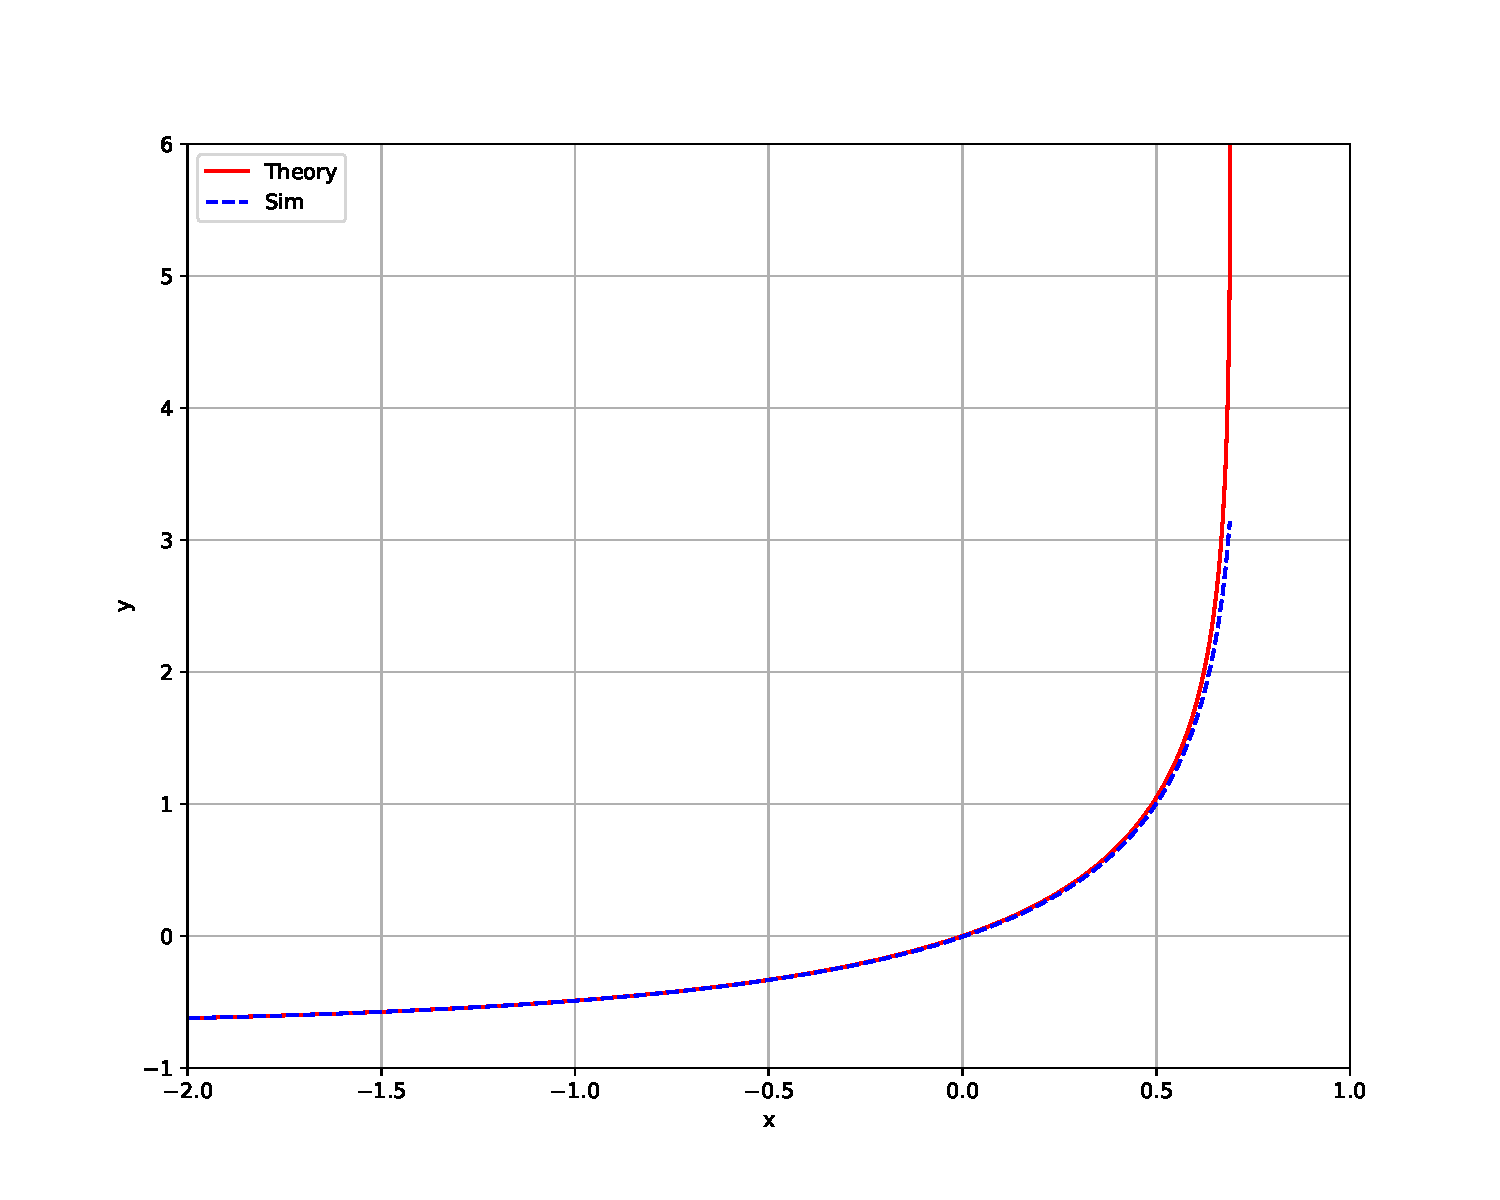
\includegraphics[width=\columnwidth]{figs/curve.pdf}
\end{figure}
\end{document}
